\begin{center}
Общее представление о системе
\end{center}

\vspace{\baselineskip}

FreeHackQuest (FHQ) -- это платформа для обучения, проведения практических занятий и соревнований по компьютерной безопасности в формате тестирования на проникновение внутри среды, моделирующей работу информационной инфраструктуры организации. FHQ включает в себя учебник, различные задачи для решения, связанные с администрированием, криптографией, компьютерно-криминалистической экспертизой, стеганографией и многими дргуими направлениями информационной безопасности.\par

\begin{center}
Компоненты системы
\end{center}

\vspace{\baselineskip}

Структура системы представлена на рисунке \ref{img:1}:
\begin{figure}[h!]
    \centering
    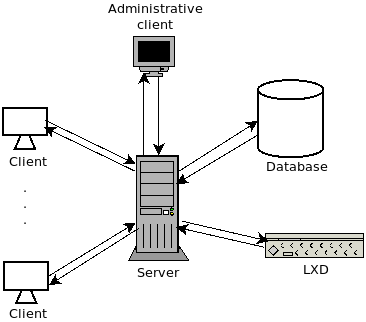
\includegraphics[width=0.65\textwidth]{1}
    \caption{Структура системы}
    \label{img:1}
\end{figure}
Система состоит из следующих компонентов:
\begin{enumerate}
\item Уровень 1: Сервер.
\item Уровень 1: LXD (сервер виртуальных машин).
\item Уровень 1: MySQL (сервер баз данных).
\item Уровень 1: Клиент.
\item Уровень 1: Административный клиент.
\end{enumerate}
